\section{Correlations in the 2D Ising Model}

Consider a 2D lattice of atoms in the presence of a \(z\)-directed magnetic field of strength
\(B\). Suppose that all atoms are identical spin-\(1/2\) systems.
We define the lattice in Snippet~\ref{lst:lattice},
where it is a \code{Matrix} containing spins of values \(s_i = 1\) (spin up) or
\(s_i = -1\) (spin down), where \(s_i\) is (twice) the \(z\)-component of the \(i\)th
atomic spin. The total energy of the system is written as:
%
\begin{equation}
    E = -J \sum_{\langle i j \rangle} s_i s_j - B \sum_{i} s_i,
\end{equation}
%
where \(J\) is the exchange energy.

\begin{algorithm}
    \caption{Define the 2D lattice for the Ising model.}
    \label{lst:lattice}
    \begin{juliacode}
        struct Lattice{T} <: AbstractMatrix{T}
            spins::Matrix{T}
        end
    \end{juliacode}
\end{algorithm}

And for different simulation algorithms, we define several types, as in
Snippet~\ref{lst:alg}, where \code{Basic} is the simplest algorithm
denoting flipping spins one by one, and \code{SwendsenWang} is the cluster
algorithm we will discuss below.

\begin{algorithm}
    \caption{Different simulation algorithms.}
    \label{lst:alg}
    \begin{juliacode}
        abstract type Algorithm end
        struct Basic <: Algorithm end
        struct Checkerboard <: Algorithm end
        struct SwendsenWang <: Algorithm end
    \end{juliacode}
\end{algorithm}

The \code{Basic} algorithm, as in Snippet~\ref{lst:basic},
is the slowest one when doing the simulation. However, it is easy to implement
and less error-prone.

\begin{algorithm}
    \caption{The simplest algorithm: flipping spins one by one.}
    \label{lst:basic}
    \begin{juliacode}
        function simulate!(lattice::Lattice, β, J, B, ::Basic)
            for index in eachindex(lattice)
                trial_spin = flipspin!(lattice, index)  # Trial move
                eᵢ_old = energy(lattice, index, J, B)
                eᵢ_new = energy(sum(neighborspins(lattice, index)), trial_spin, J, B)
                P = exp(-β * (eᵢ_new - eᵢ_old))
                if P > rand()
                    lattice[index] = trial_spin  # Accept the trial move
                end
            end
            return lattice
        end
    \end{juliacode}
\end{algorithm}

\begin{figure}[hbt]
    \centering
    \begin{subfigure}{0.49\textwidth}
        \centering
        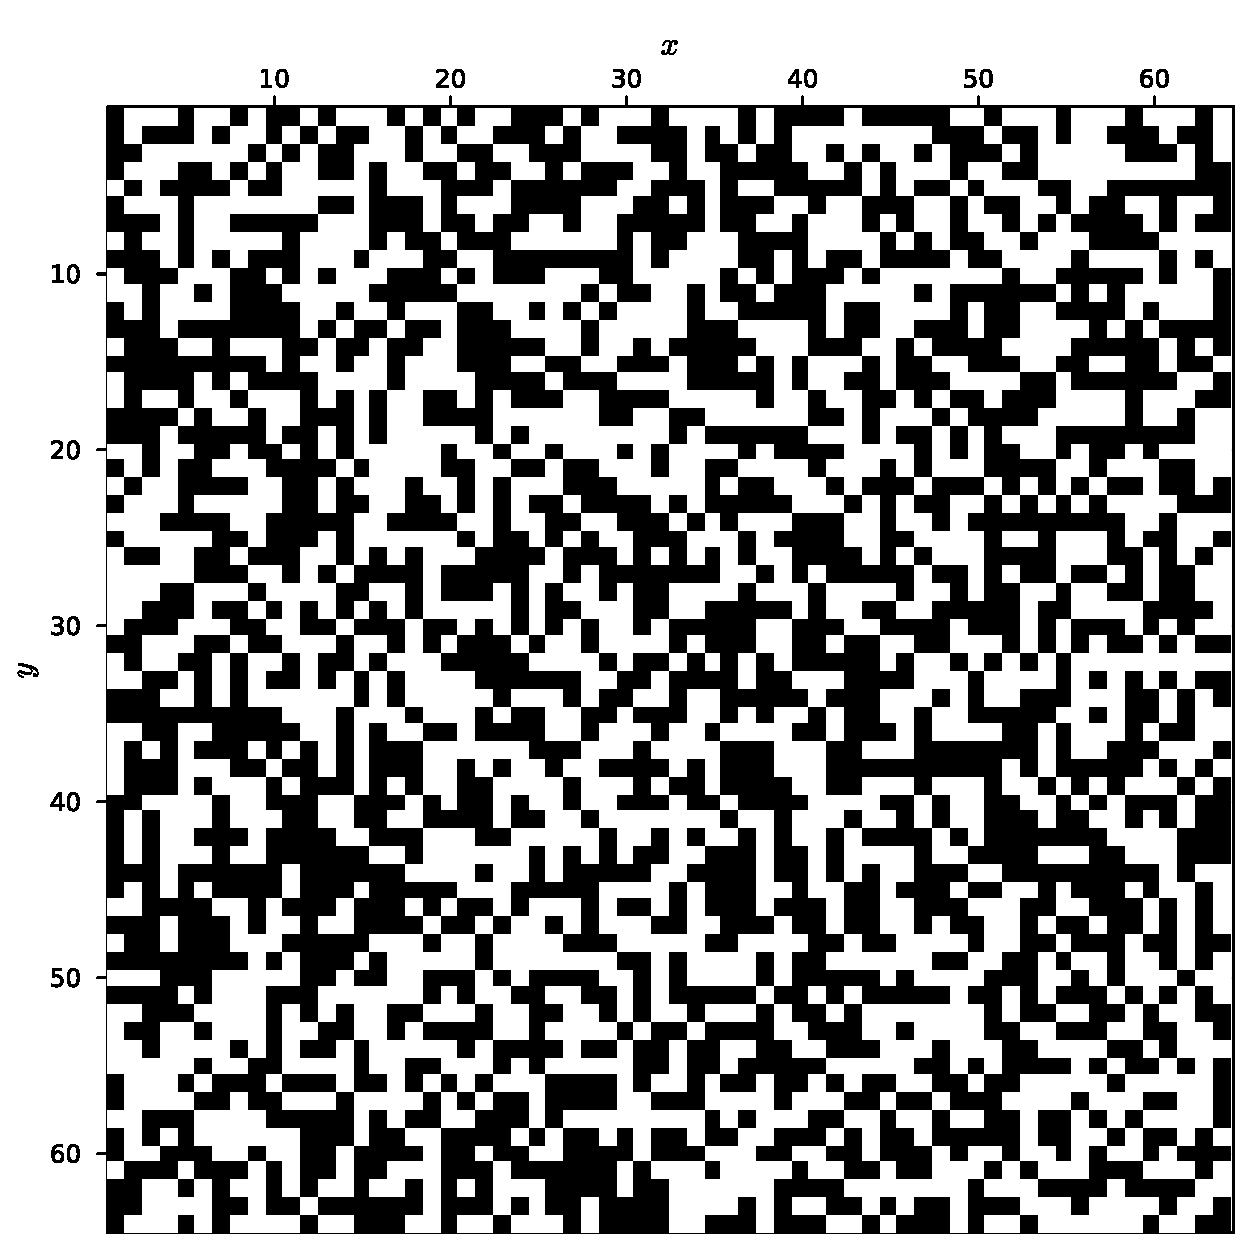
\includegraphics[width=\linewidth]{basic_J=0.455_t=0}
    \end{subfigure}
    \hfill
    \begin{subfigure}{0.49\textwidth}
        \centering
        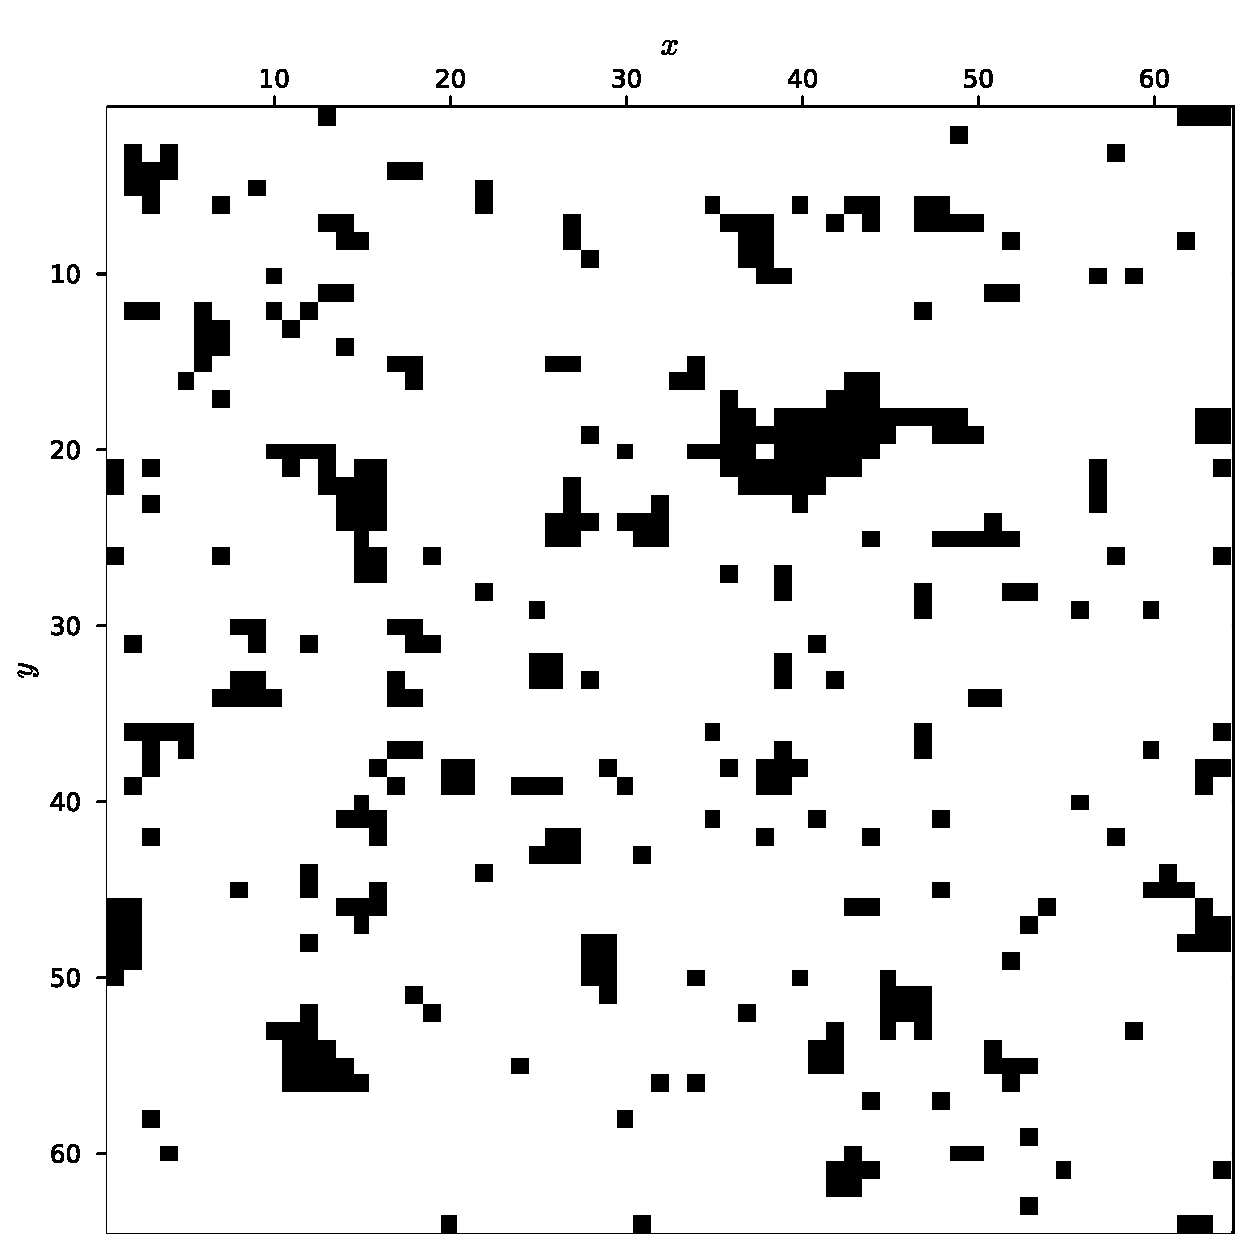
\includegraphics[width=\linewidth]{basic_J=0.455_t=5000}
    \end{subfigure}
    \caption{Magnetization pattern of a \(64 \times 64\) array of ferromagnetic atoms in the
        absence of an external magnetic field at \(t = 0\) (left), and \(t = 5000\) (right,
        thermal equilibrium), with \(J = 0.455\). Black/white squares indicate spin up and
        spin down, respectively. The simulation is done using the \code{Basic} algorithm.}
    \label{fig:rand_J=0.455}
\end{figure}

The Metropolis--Hastings approach to the Ising model, which completely avoids the use of the mean
field approximation, is based on the following algorithm, i.e.,
step through each atom in the array in turn:
%
\begin{itemize}
    \item For a given atom, evaluate the change in energy of the system, \(\Delta E\), when
          the atomic spin is flipped.
    \item If \(\Delta E < 0\) (lowering energy), then flip the spin.
    \item If \(\Delta E > 0\) then flip the spin with probability
          \(P=\exp\bigl(-\beta \Delta E\bigr)\).
\end{itemize}
%
Repeat the process many times until thermal equilibrium is achieved.

In Snippet~\ref{lst:basic}, we use function \code{neighborspins} to find all the neighboring
spins \(s_j\) of a specific spin \(s_i\). Notice we do not update the spin immediately
since it is just a trial move at the beginning. We only update it until the probability of
the flipping is larger than a (uniformly distributed between \(0\) and \(1\)) random number.
Since for any fixed \(P\), the probability of generating a random number that is smaller
than \(P\) is \(P\). Therefore, we accept the trial move with probability \(P\).

We plot the results of one simple simulation in Figure~\ref{fig:rand_J=0.455},
with the initial spins randomly chosen.
As we can see, since the temperature is lower than \(T_c\) (\(J > J_c\)),
the system will converge to an equilibrium state where there is net magnetization.
That is, most of the spins on the right are down (white).
If we plot the magnetization, which is the average value of the spins as a function
of simulation timesteps, as shown in Figure~\ref{fig:mag_J=0.455}.
The mean value of the magnetization after thermalization is around \(-0.78\).

\begin{figure}[hbt]
    \centering
    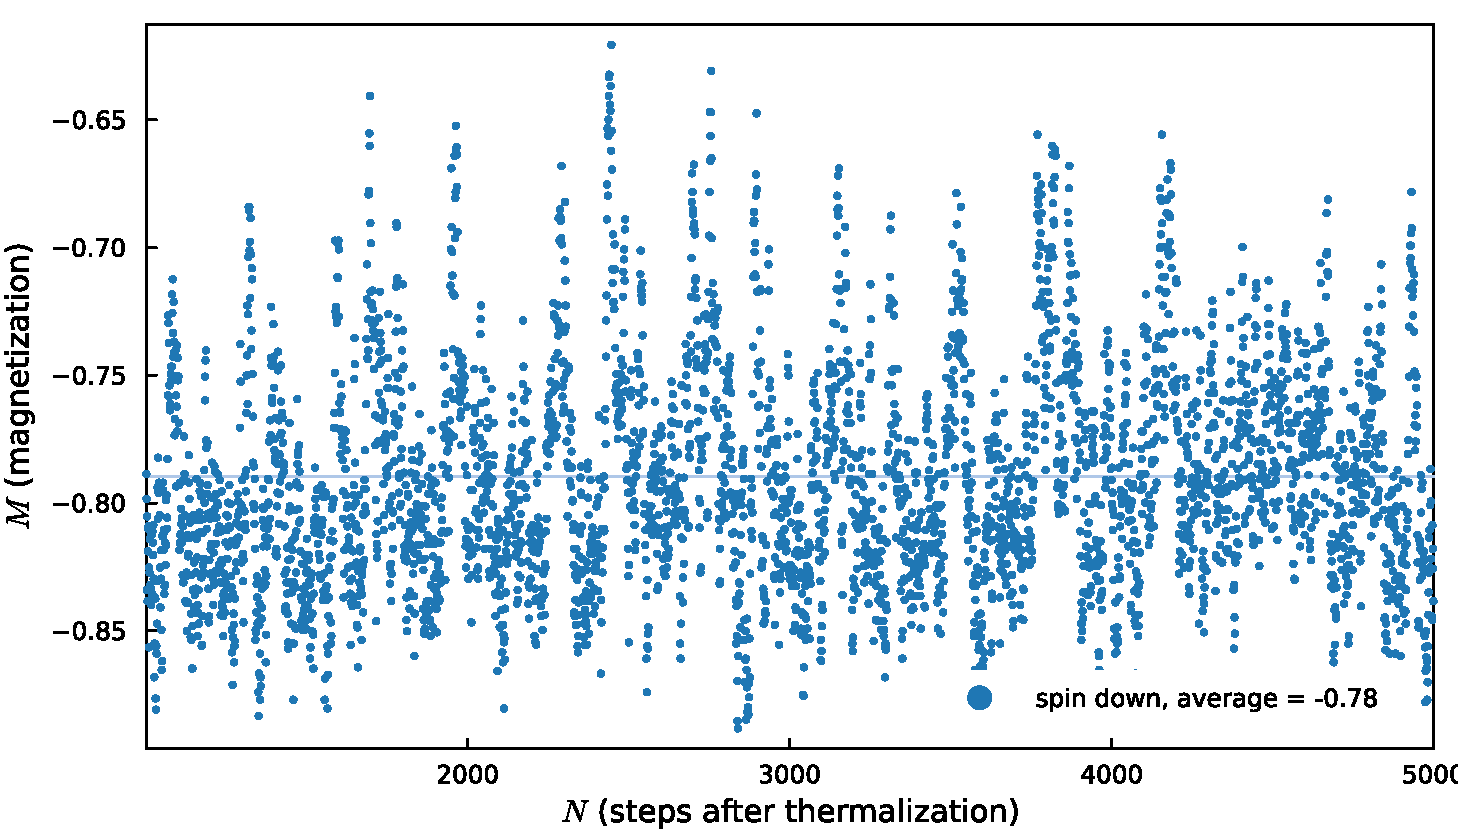
\includegraphics[width=0.9\textwidth]{basic_J=0.455_mag_t>1000}
    \caption{Magnetization of a \(64 \times 64\) array of ferromagnetic atoms in thermal
        equilibrium and in the absence of an external magnetic field as a function of
        simulation timesteps (\(t\) from \(1000\) to \(5000\)). The temperature is below the
        critical temperature. The mean value of the magnetization after thermalization is
        plotted in a lighter color.}
    \label{fig:mag_J=0.455}
\end{figure}

\begin{figure}[hbt]
    \centering
    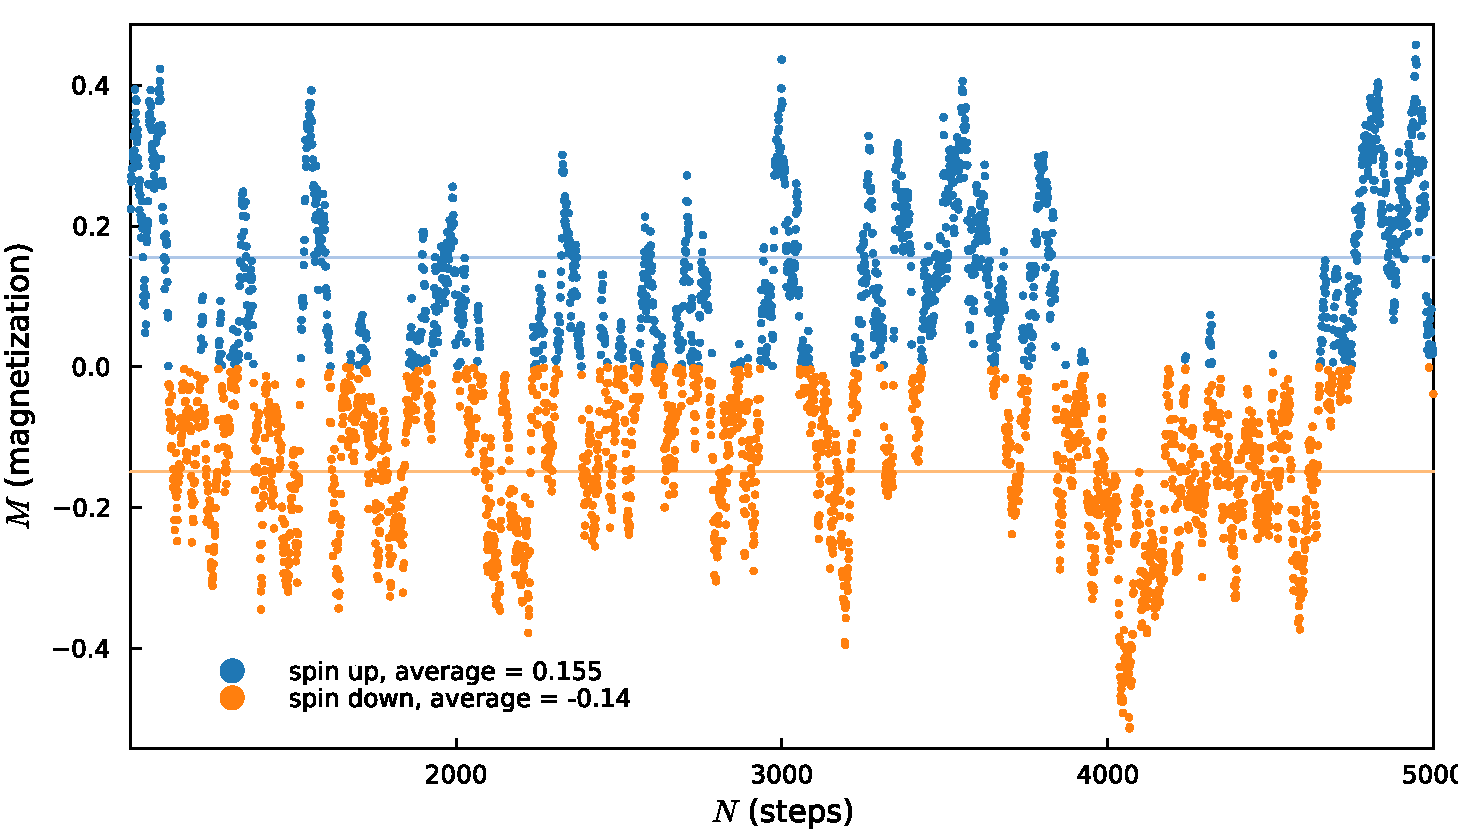
\includegraphics[width=0.9\textwidth]{basic_J=0.41_mag_t>1000}
    \caption{Magnetization of a \(64 \times 64\) array of ferromagnetic atoms in thermal
        equilibrium and in the absence of an external magnetic field as a function of
        simulation timesteps (\(t\) from \(1000\) to \(5000\)). The temperature
        (\(J = 0.41\)) is well above the critical temperature. The mean value of the
        magnetization after thermalization is plotted in a lighter color.}
    \label{fig:mag_J=0.41}
\end{figure}

Now, we select a temperature that is well above the critical temperature \(T_c\),
i.e., \(J < J_c\), to see how the system evolves as a function of time.
For example, we choose \(J = 0.41\). At this temperature, the net magnetization should
be \(0\). We expect a magnetization pattern where the black (up) and
white (down) spins have roughly the same number after thermalization.
The initial lattice we chose is an all-black pattern. That is, the net magnetization
is \(1\). We let it evolve and see how thermal fluctuations turn the lattice into
a system with zero net magnetization.
We plot the magnetization as a function of time in Figure~\ref{fig:mag_J=0.41}.
As it shows, the mean value of spin-up is \(0.155\), and that of spin-down is \(-0.14\).
So the total mean value will be around \(0\), as expected.

However, if we select a temperature that is not that far from the critical temperature,
we may have net magnetization larger than zero even after \(5000\) steps.
For example, now we choose \(J = 0.435\), which is close to \(J_c\), and redo the
simulation.
If we plot the magnetization as a function of time in Figure~\ref{fig:mag_J=0.435},
we can see even after \(5000\) steps, the values of spin-up and spin-down still do
not converge. Thus, no thermal equilibrium is achieved in this time evolution.
In conclusion, we are observing the critical slowing down of the \code{Basic}
Metropolis algorithm.

\begin{figure}[hbt]
    \centering
    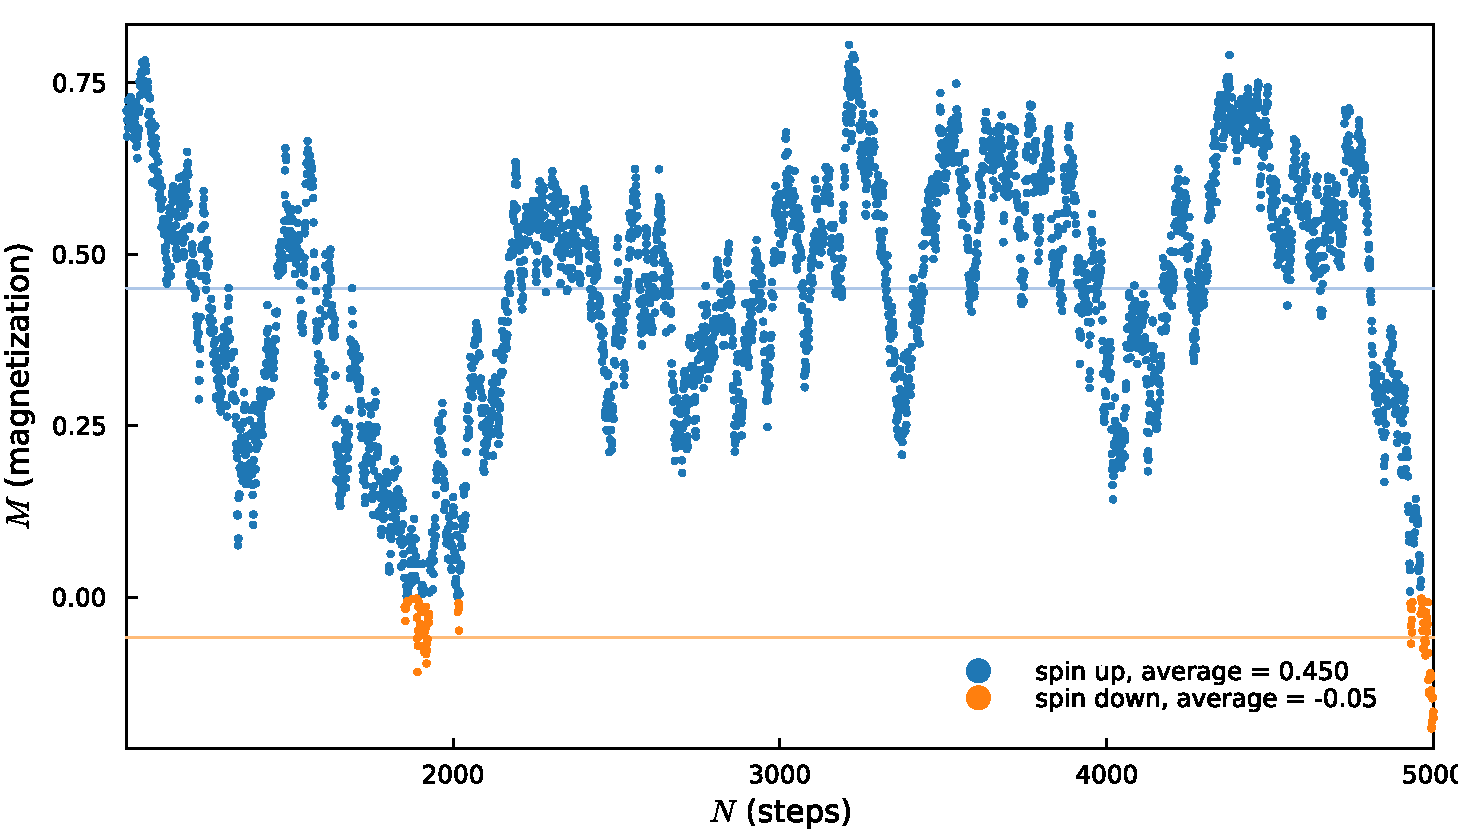
\includegraphics[width=0.9\textwidth]{basic_J=0.435_mag_t>1000}
    \caption{Magnetization of a \(64 \times 64\) array of ferromagnetic atoms in the absence
        of an external magnetic field as a function of simulation timesteps (\(t\) from
        \(1000\) to \(5000\)). The temperature (\(J = 0.435\) is only a little higher than
        the critical temperature. The mean values of the magnetization of these steps are
        plotted in lighter colors. No thermal equilibrium is achieved within \(5000\)
        steps.}
    \label{fig:mag_J=0.435}
\end{figure}

\begin{figure}[hbt]
    \centering
    \begin{subfigure}{0.49\textwidth}
        \centering
        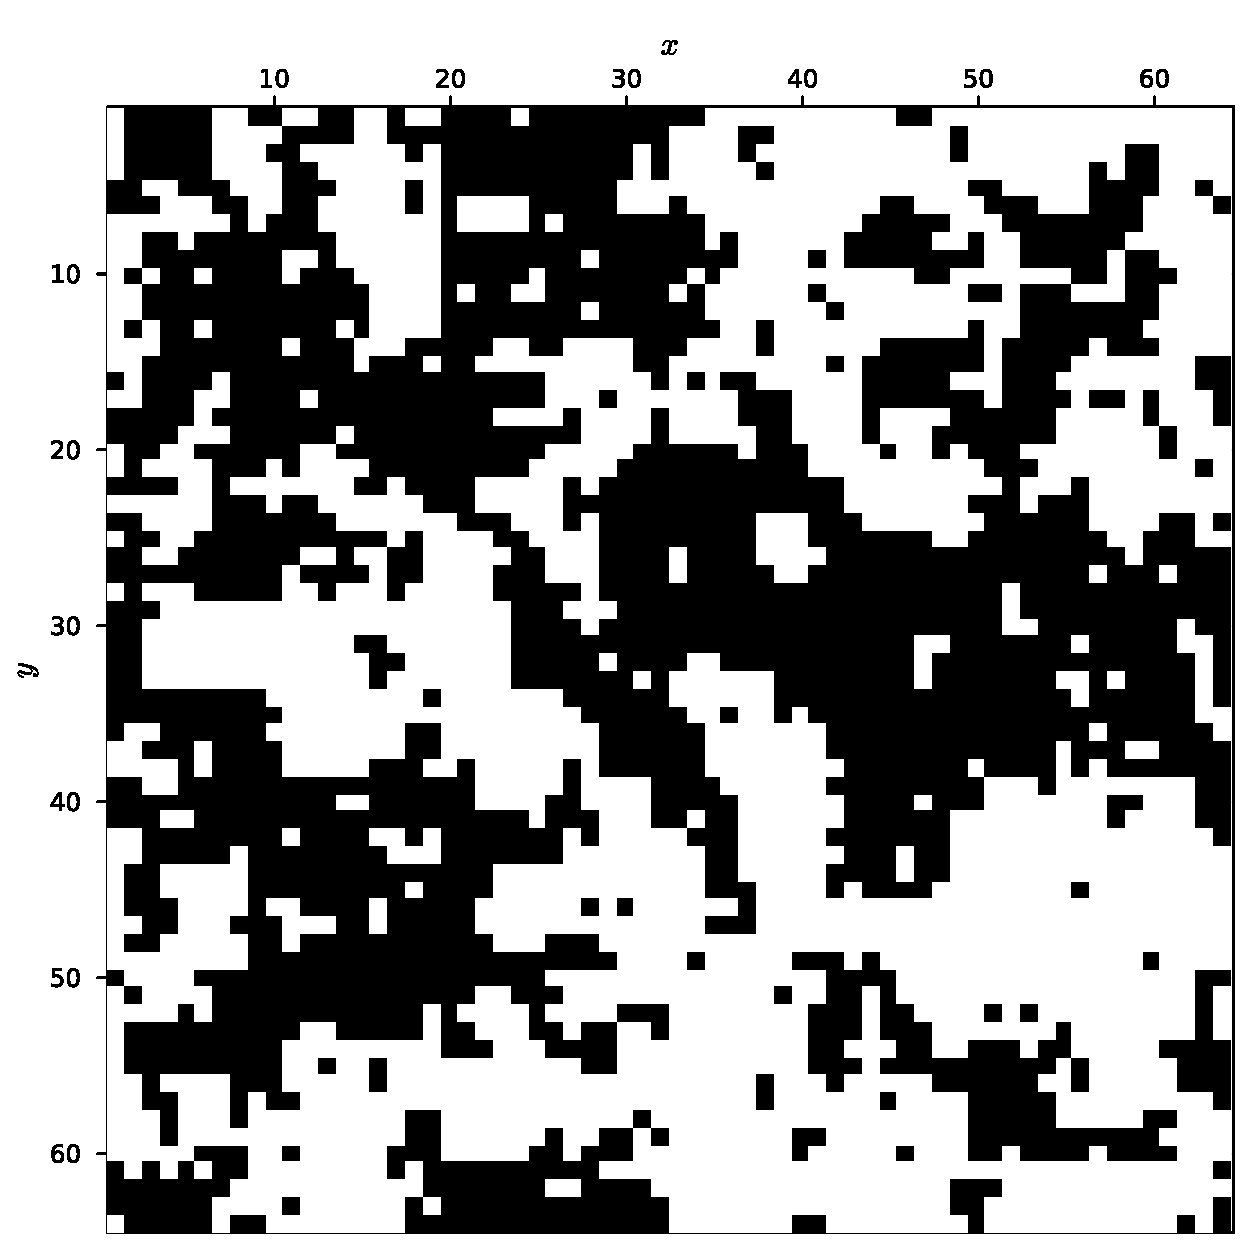
\includegraphics[width=\linewidth]{basic_J=0.41_t=5000}
    \end{subfigure}
    \hfill
    \begin{subfigure}{0.49\textwidth}
        \centering
        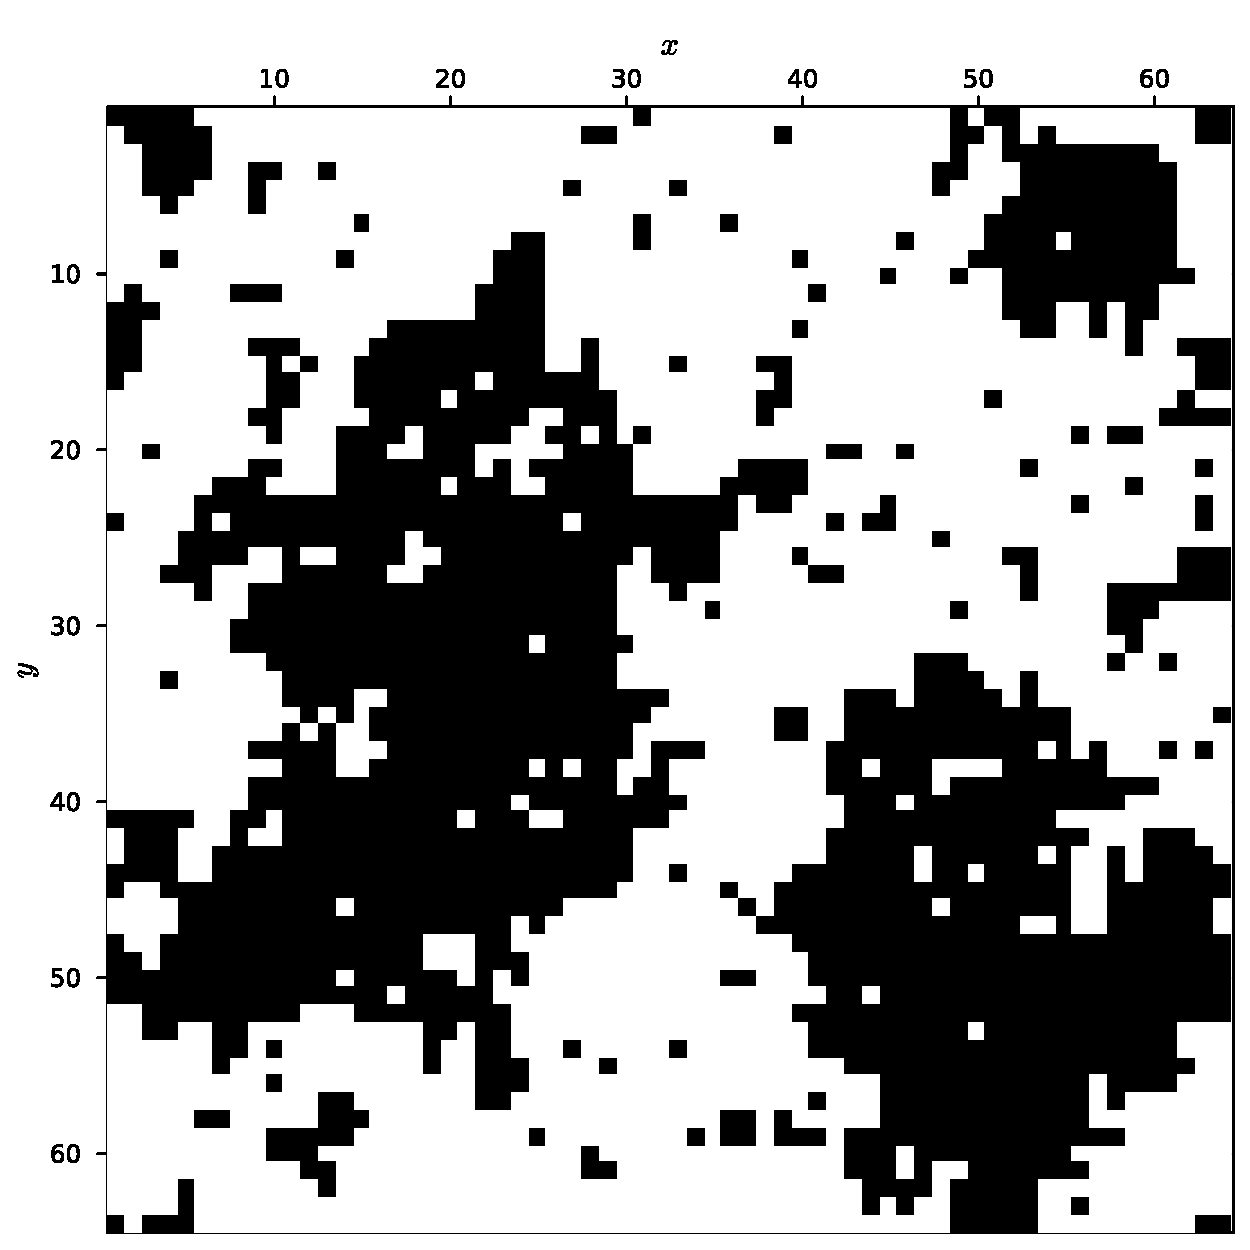
\includegraphics[width=\linewidth]{basic_J=0.435_t=5000}
    \end{subfigure}
    \caption{Magnetization pattern of a \(64 \times 64\) array of ferromagnetic atoms in the
        absence of an external magnetic field at \(t = 5000\), with \(J = 0.41\) (left) and
        \(J = 0.435\) (right).}
    \label{fig:t_5000}
\end{figure}

We plot the magnetization patterns of the lattice at \(t = 5000\) for both \(J\) values
mentioned above in Figure~\ref{fig:t_5000}. As we can see, for the \(J = 0.41\) case, the
distribution of up and down spins are more uniform, while for the \(J = 0.435\) case, there
are clearly clusters of up and down spins, leading to net magnetization.

\begin{algorithm}
    \caption{The Swendsen--Wang algorithm for simulating the Ising model.}
    \label{lst:cluster}
    \begin{juliacode}
        function simulate!(lattice::Lattice, β, J, B, ::SwendsenWang)
            index = rand(CartesianIndices(lattice))
            P = 1 - exp(-β * (2J + B))
            recursive_flipspin!(lattice, index, lattice[index], P)
            return lattice
        end
    \end{juliacode}
\end{algorithm}

As the Ising model approaches its critical point, the size of spatial clusters grows. It is
this growth in the average size of clusters responsible for diverging correlation
length at \(T_c\) and the corresponding second-order phase transition. The cluster algorithm
avoids the critical slowing down that comes from the slow evolution through phase space of
the simple, local site Metropolis algorithm.

For the cluster algorithm, we need to adopt a recursive scheme, as shown in
Snippet~\ref{lst:cluster}. The recursive spin-flipping method is defined in
Snippet~\ref{lst:recur}.

In each timestep, we randomly select one atom, flip its spin, and for each of its four
neighbors, see if it has a ``link'' connecting the spins (i.e., the ``bond'' is \emph{open}).
If so, flip that spin with probability \(P = 1 - \exp(-2J)\).
Recursively repeat these steps until we have reached the end of the tree where
every ``bond'' is closed.

\begin{algorithm}
    \caption{The recursive spin-flipping method.}
    \label{lst:recur}
    \begin{juliacode}
        function recursive_flipspin!(lattice::Lattice, index, spin₀, P)
            spin = flipspin!(lattice, index)
            for index′ in findneighbors(lattice, index)
                if lattice[index′] == spin₀ && P > rand()
                    recursive_flipspin!(lattice, index′, spin₀, P)
                end
            end
            return spin
        end
    \end{juliacode}
\end{algorithm}

\begin{figure}[hbt]
    \centering
    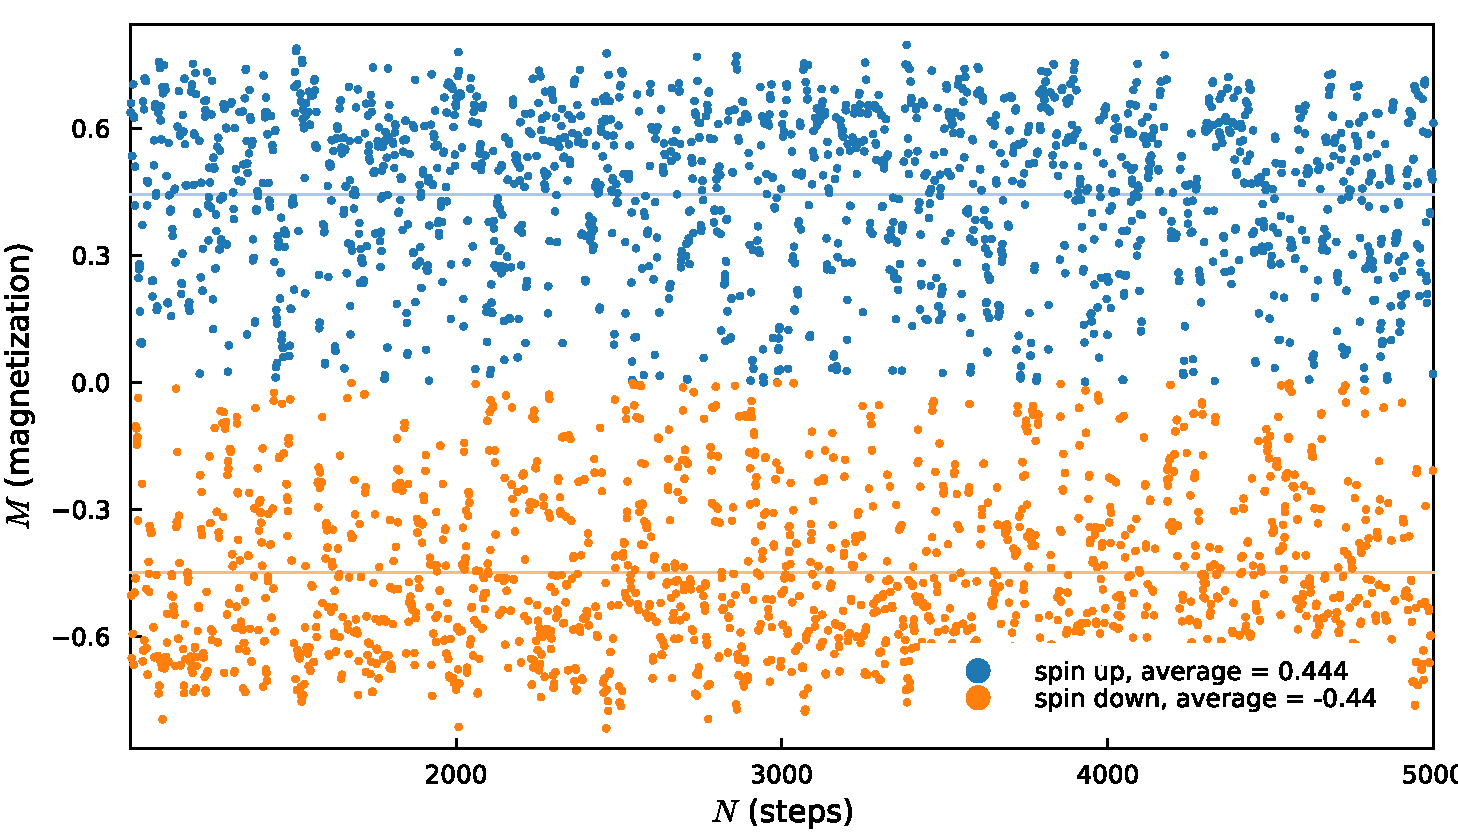
\includegraphics[width=0.9\textwidth]{cluster_J=0.435_mag_t>1000}
    \caption{Magnetization of a \(64 \times 64\) array of ferromagnetic atoms in the absence
        of an external magnetic field as a function of simulation timesteps (\(t\) from
        \(1000\) to \(5000\)). The temperature (\(J = 0.435\)) is only a little higher than
        the critical temperature. The mean values of the magnetization of these steps are
        plotted in lighter colors. The simulation is done using the \code{SwendsenWang}
        algorithm.}
    \label{fig:mag_J=0.435_cluster}
\end{figure}

Then we use the cluster (Swendsen--Wang) algorithm to calculate the magnetization as a
function of time for the \(J = 0.435\) case. The results are plotted in
Figure~\ref{fig:mag_J=0.435_cluster}. As shown in the figure, the magnetization is rapidly
switching between net positive and negative states, and the averages of these states are
\(0.444\) and \(-0.44\), converging to zero much faster than the \code{Basic} algorithm.
